\documentclass[a4paper]{article}

%% Language and font encodings
\usepackage[english]{babel}
\usepackage[utf8x]{inputenc}
\usepackage[T1]{fontenc}

%% Sets page size and margins
\usepackage[a4paper,top=3cm,bottom=2cm,left=3cm,right=3cm,marginparwidth=1.75cm]{geometry}

%% Useful packages
\usepackage{amsmath}
\usepackage{graphicx}
\usepackage[colorinlistoftodos]{todonotes}
\usepackage{hyperref}

\title{Book Bot Project}
\author{Group 7}

\begin{document}
\maketitle

\begin{abstract}
This file is a project report about Group 7's Book Bot Project for CmpE451 class. Information in this file is up to Milestone 1.
\end{abstract}

\section{Project Description}

 \qquad Book Bot Project is an assistant that can help users with everything related to books. It is a bot, and it works via Telegram. Working via Telegram makes the bot more accessible; users don't need to install anything extra and it is cross platform. \\
  
  
  \quad The base and most important functionality is to communicate with natural language. The bot can carry on a conversation with daily English. \\
 
  
  \quad Users can ask the bot about books. They can search books with different keywords, genres or authors, they can filter them in any way they want and they can sort them. They also can get information about specific books, see its current popularity via ratings or read the comments about the book.\\
 
  
  \quad Users can also give the bot feedback about the books they have read. They can comment on a book or rate a book. This will help the bot learn more about what the user likes and help it work more user oriented \\
 
  
  \quad The bot can also recommend the user some books depending on their previous ratings and taste of books.

\subsection{Project Requirements}

We have defined our project requirements as follows and our customer has agreed and approved the requirements. Note that the following is a summary of the detailed requirements page. You can see the full list from \href{https://github.com/bounswe/bounswe2017group7/wiki/Project-Requirements}{project requirements} in our wiki page.

\begin{enumerate}
\item Functional Requirements
  \begin{enumerate}
  \item System Requirements
    \begin{enumerate}
    \item Telegram will be the medium for the bot.
    \item Goodreads or Google Books will be our source of book related information.
    \item Wit.ai will be used for NLP purposes to understand natural language.
    \item There will be regular users, admins and moderators.
    \item There will be a conversation tree which is going to be used to determine the conversation direction.
    \end{enumerate}
  \item User Requirements
    \begin{enumerate}
    \item We will have regular users as Telegram Users.
      \begin{enumerate}
        \item Users will be able to get information; search for books, filter them, sort them and read comments about them
        \item Users will be able to give feedback about books; comment on them and rate them.
        \item Users will be able to get book recommendations.
        \end{enumerate}
    \item We will have admin users.
        \begin{enumerate}
        \item Admins will be able to modify the conversation tree
        \item Admins will be able to see and flag comments
        \item Admins will be able to see and block users
        \end{enumerate}
    \item We will have moderator users.
        \begin{enumerate}
        \item Moderators will be able to see and flag comments
        \item Moderators will be able to see and block users
        \end{enumerate}
    \end{enumerate}
  \end{enumerate}
\item Non Functional Requirements
  \begin{enumerate}
  \item Speed: We are creating a bot which users can chat with so the response time cannot be more than 5 seconds.
  \item Size: We want our bot to be portable an not bulky, we will use the Telegram as our medium hence the user won't need extra space for the bot.
  \item Usage: It should be easy to use, there shouldn't be any training time.
  \item Requirements: Bot needs internet connection to work.
  \item Failures: If bot fails, it shouldn't take more than ten minutes to restart the system and get it working again.
  \item Target devices: We are targeting all platforms in which Telegram works.
  \item User Satisfaction: Bot should keep track of the success of its recommendations by tracking the ratings of the recommended books.
  \end{enumerate}
\end{enumerate}
\newpage

\subsection{Project Design}

See \autoref{fig:design}

\begin{figure}[!hb]
  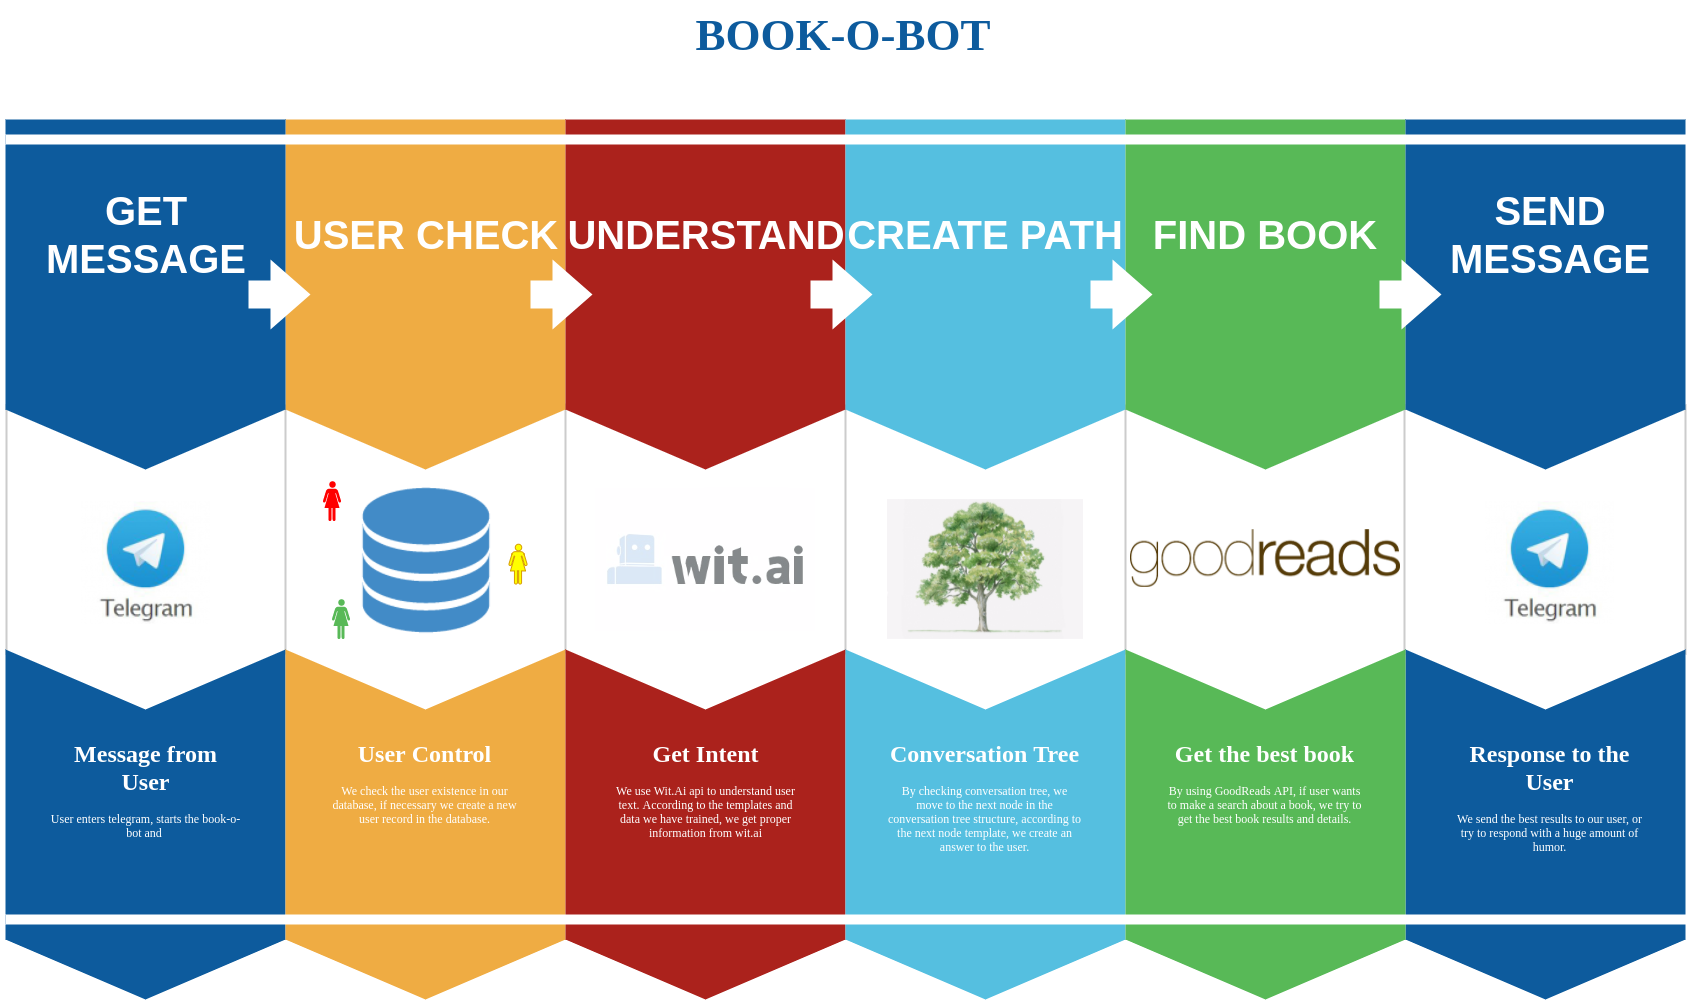
\includegraphics[width=\linewidth]{figures/design.png}
  \caption{Project Design}
  \label{fig:design}
\end{figure}


\newpage

\subsection{Project plan}

TODO: write project plan. It is going to be in tabular form. See Table~\ref{tab:projectplan}

\begin{table}
\centering
\begin{tabular}{l|r}
Row Name & Row Name \\\hline
Column Name & column value \\
Column Name & column value
\end{tabular}
\caption{\label{tab:projectplan}An project plan table.}
\end{table}

\section{Project Milestones}
\subsection{Milestone 1}
Book bot works fine for getting information purposes. (End of October)
\subsection{Milestone 2}
Book bot works fine for giving information purposes. (End of November)
\subsection{Final Milestone}
Book bot is able to recommend books. (Project is finished)

\section{Project status}
\subsection{Deliverable List}

\begin{enumerate}

   \item  Goodreads API
   
   \item  Telegram API  
     
   \item  Node/Conversation Graph
    
   \item Database Creation  
   
  \item   Cloud
  
  \item Telegram Service(Cloud)

   
  \item   Sign-up/Login
  
  \item   Settings
  
  \item Admin Dashboard
  
    \item Viewing Conversation Graph
      \item Testing Demo  
      
 \end{enumerate}

\subsection{Deliverable Status}
TODO: write deliverable status. It is going to be in tabular form. See Table~\ref{tab:deliverablestatus}

\begin{table}
\centering
\begin{tabular}{l|r}
Row Name & Row Name \\\hline
Goodreads API & Delivered \\
Telegram API & Delivered \\
Node/Conversation Graph & Delivered \\
Database Creation  & Delivered \\
Cloud(AWS) & Partially Delivered \\
Sign-up/Login & Partially Delivered \\
Settings & Not Delivered\\
Admin Dashboard & Partially Delivered \\
Viewing Conversation Graph & Delivered \\
Testing Demo & Partially Delivered
\end{tabular}
\caption{\label{tab:deliverablestatus}An deliverable status table.}
\end{table}

\subsection{Deliverable Evaluation}
\begin{enumerate}
\item Goodreads API
\begin{enumerate}
  \item It is delivered however we may change this API to Google Books due to latency problems.
   \end{enumerate}
   \item  Telegram API
   \begin{enumerate}
    \item It is done and since it was the main thing to communicate with users, it was crucial. We build whole structure onto it.
     \end{enumerate}
   \item  Node/Conversation Graph
   \begin{enumerate}
    \item We have done this, it works properly. The conversation graph is traversed while conversation.
   \end{enumerate}
   \item Database Creation  
   \begin{enumerate}
   \item The database models are created as designed in the design plan.
  \end{enumerate}
  \item   Cloud(AWS)
  \begin{enumerate}
 \item Cloud(AWS) is set up however we couldn't make it work exactly, as it is on our local.
  \end{enumerate}
  \item   Sign-up/Login
  \begin{enumerate}
  \item It is delivered with the help of DJango interface. We may need to customize this to our needs in the future. 
  \end{enumerate}
  \item   Settings
  \begin{enumerate}
 \item  We couldn't find energy and time to implement this part. It will be ready on the 2nd milestone. This wasn't on the critical path , so it isn't a big deal to being this deliverable is not delivered.
  \end{enumerate}
  \item Admin Dashboard
  \begin{enumerate}
 \item  It is delivered with the help of Mptt interface. We may need to customize this to our needs in the future. 
    \end{enumerate}
    \item Viewing Conversation Graph
    \begin{enumerate}
  \item It is delivered and it was necessary to see conversation trees structure.
      \end{enumerate}
      \item Testing Demo
      \begin{enumerate}
    \item  We couldn't tested the demo version very well, we planned to put our internal milestone 3 days before the customer milestone to prevent this happen again.
      \end{enumerate}
      \end{enumerate}
\newpage
\section{Coding Work}
You can find each team member's contribution to the code in the ~\autoref{tab:codingwork}

\begin{table}[!hb]
\centering
\begin{tabular}{l|r}
Name & Coding Work \\\hline
Salih Sevgican & GoodReads API implementation \\ 
 & book API class for ease of use \\
 & Main Page of the project (Front End)\\
 & AWS has been configured for the deployment\\
 & Updated requirements.txt\\
 & GoodReads compatibility with TelegramBot tested on telegramapi\\\hline
Irmak Kavasoglu & Initial environment setup for Django \\
& Setting up database model for Telegram User \\
& Setting up database model for Templates \\
& Setting up database model for Conversation Node \\
& Integrating Mptt tool for conversation tree \\
& Registering models to admin page and customizing their look \\\hline
Ali Goksu Ozkan & Implementing GET/POST to functionalize Node class \\
& Implementing GetNextNode class to function Conversation Tree \\
&  Conversation Tree integration with Telegram API\\
&  Conversation Tree compatibility with wit.ai\\\hline
M. Melih Mutlu & Telegram API implementation \\ 
 & Writing GET and POST methods for our API \\
 & Integrating Telegram bot with Wit.ai\\
 & Deploying the project to AWS \\
 & Node change operations for Telegram User \\\hline
Taha Kucukkatirci & Wit.ai API configuration \\
& Intents have been defined and trained with some training inputs\\
& Implementation of getIntent method \\
& Implementation of the method to auto train Wit.ai app \\
& Validation of the requests from users and retrain by them if valid \\\hline
Add your name & add your contribution
\end{tabular}
\caption{\label{tab:codingwork}Coding work table.}
\end{table}

\section{Evaluation of tools and managing the project}
\subsection{Django}
Django is a free and open-source Web framework implemented for Python. It led us writing your back-end without needing to reinvent the wheel. Since Django's primary goal is to ease the creation of complex, database-driven apps, we decided to use it. It was also in the emerging technologies according to our software tool research. It was easy to learn, install and set configuration.

Ridiculously fast.
\subsection{Mptt}
MPTT is a API to store hierarchical data in a database. The purpose of the tool is to make retrieval operations efficient. We needed a conversation tree in our software structure. But implementing tree structure was a little unefficient for us. We needed to visualize the tree for the admin use and we needed other functions such as get\_Children. We thought that we could focus on the functional details rather performance or implementation details of the tree. Therefore we decided to use this API. The API was very useful and made our job on the conversation tree easy. What we learned from this experience is utilizing a functional and well-implemented API would make your project management better.

\subsection{Telegram}
Telegram offers HTTP-based interface to do most of the operations that we could need for a chat bot. Receiving and sending messages are the ones that we had to implement in first place. Telegram API provides all messages that the bot received in last 24 hours. For this reason, we had to careful to not processing same messages more than once. Response time of Telegram API is satisfying so far. As far as we read in documentation, Telegram API supports actions that we will need for this projects. However we haven't used it for sending and receiving more complicated messages such as book results that includes images, links or buttons. 
\subsection{Wit}

\quad Wit.ai is a service provided by Facebook for intent detection. It is a very useful tool and makes our job much easier. First of all, we created our app on Wit.ai and then defined our intents and train them with some training sentences. After enough training data, it gets an insight about the data and catches the patterns for each intent. Then, it detects the intent of the unseen, new sentences easily. Like said before, it is a very useful tool and speed up our project by handling intent detection issue. We will also use it for further purposes like getting and remembering context of the conversation and this will make our bot answer in a more coherent and smarter way.
\subsection{GoodReads}

\quad GoodReads API is very useful to make a search about a book by given any kind of keyword. Keyword can be related to author, genre or title, doesn't matter, this api makes a succesfull search every time. We've used a wrapper library for GoodReads API which made easy to write methods for search types. Library is a litlle bit complicated despite it is written to ease our job. Unfortunately not every book is being hold as a same type in goodreads database, some of queries returns arrays with additional information of book such as order number of a book in the book series, and some of queries returns just the name of book. This is an issue we need to handle very well in order to make a great impression with the responds to the bot user.  
\subsection{AWS}

\quad AWS is the service that we use for our project's server need. It is very convenient to start an instance and easy to use. Connection to the Amazon server is very easy on Ubuntu and our group members mostly use Ubuntu. On Ubuntu, by ssh, we can connect to the Amazon server with one line command.We first created an AWS account and then waited for approval of initial payment. Then we launched an EC2 instance on ubuntu and we are given a .pem file. We stored it in a folder and changed its privacy by chmod 400 command. Lastly, we achieved to connect server with given AWS id and ip by ssh on ubuntu. We sent the .pem file to other group members and told the process to them to make them able to connect to the server. For running our project easily, we changed our ip as elastic ip. We sent our ip address that is associated with our AWS account to all members. So we can mask the failure of an instance by instantly remapping the address to another instance. 

\section{Summary}
TODO fill

\end{document}
